\documentclass{article}
\usepackage[UTF8]{ctex}  % 使用中文支持包
\usepackage[a4paper, margin=1in]{geometry}  % 设置纸张大小和边距
\usepackage{anyfontsize}  % 解决字体大小报错问题
\usepackage{fancyhdr}  % 设置页眉、页脚、页码
\usepackage{lscape}
\usepackage{longtable}  % 支持长表格
\usepackage{booktabs}
\usepackage{graphicx}
\usepackage{colortbl}
\usepackage{tabularx}
\usepackage{multirow}
\usepackage[table,xcdraw]{xcolor}

\usepackage{amsmath}  % 数学公式支持
\usepackage{cases}  % 支持联立编号
\usepackage[sort]{natbib}  %国标参考文献 with sorting option

\usepackage{graphicx}  % 插入图片支持
\usepackage{float}  % 设置图片浮动位置
\usepackage{subfigure}  % 插入多图时用子图显示

\usepackage{listings}  % 代码块支持
\usepackage{xcolor}  % 设置代码块颜色

\lstset{
    basicstyle          =   \sffamily,          % 基本代码风格
    keywordstyle        =   \bfseries,          % 关键字风格
    commentstyle        =   \rmfamily\itshape,  % 注释的风格,斜体
    stringstyle         =   \ttfamily,  % 字符串风格
    flexiblecolumns,                % 别问为什么,加上这个
    numbers             =   left,   % 行号的位置在左边
    showspaces          =   false,  % 是否显示空格,显示了有点乱,所以不现实了
    numberstyle         =   \zihao{-5}\ttfamily,    % 行号的样式,小五号,tt等宽字体
    showstringspaces    =   false,
    captionpos          =   t,      % 这段代码的名字所呈现的位置,t指的是top上面
    frame               =   lrtb,   % 显示边框
}

\lstdefinestyle{Python}{
    language        =   Python, % 语言选Python
    basicstyle      =   \zihao{-5}\ttfamily,
    numberstyle     =   \zihao{-5}\ttfamily,
    keywordstyle    =   \color{blue},
    keywordstyle    =   [2] \color{teal},
    stringstyle     =   \color{magenta},
    commentstyle    =   \color{red}\ttfamily,
    breaklines      =   true,   % 自动换行,建议不要写太长的行
    columns         =   fixed,  % 如果不加这一句,字间距就不固定,很丑,必须加
    basewidth       =   0.5em,
}

\usepackage[hyphens]{url}  % 支持链接换行
\usepackage{hyperref}  % 超链接支持

\hypersetup{
    hidelinks,
    colorlinks=true,
    allcolors=black,
	pdfstartview=Fit,
	breaklinks=true
}

\usepackage{gbt7714}  %国标参考文献

\bibliographystyle{gbt7714-numerical}

\usepackage{lastpage}  % 添加lastpage包

\newcommand\f[2]{\frac{#1}{#2}}
\newcommand\pf[2]{\frac{\partial#1}{\partial#2}}
\newcommand\df[2]{\dfrac{#1}{#2}}
\newcommand\pdf[2]{\dfrac{\partial#1}{\partial#2}}
\newcommand\zsin[1]{\frac{e^{i#1}-e^{-i#1}}{2i}}
\newcommand\zdsin[1]{\dfrac{e^{i#1}-e^{-i#1}}{2i}}
\newcommand\zcos[1]{\frac{e^{i#1}+e^{-i#1}}{2i}}
\newcommand\zdcos[1]{\dfrac{e^{i#1}+e^{-i#1}}{2i}}
\newcommand\zline[1]{#1-\overline{#1}}
\newcommand\dg[2]{#1^{\circ}#2'}

\setlength{\headheight}{16pt}
\pagestyle{fancy}
\fancyhf{}

\title{\bf\huge 对比PWR和BWR蒸汽产生的异同}
\author{Jerry}
\date{\today}
\pagenumbering{arabic}

\begin{document}

\fancyhead[L]{Jerry}
\fancyhead[C]{对比PWR和BWR蒸汽产生的异同}
\fancyhead[R]{核电厂系统与设备-黄善仿}
\fancyfoot[C]{\thepage}

\maketitle
\tableofcontents

\section{堆芯结构}

\textbf{相同点}:PWR和BWR的堆芯都包含燃料元件和慢化剂,堆芯通常是垂直排列的燃料棒,利用相似的UO$_2$燃料裂变产生热量。且堆芯都是近似圆柱形,$H/D$一般在0.9到1.0之间,以减少堆芯的体积和临界质量。

\textbf{不同点}

如图\ref{fig:PWR-fuel-rod},PWR的设计为在高压环境下通过热交换向液态的冷却剂直接传递热量。由于压水堆一般工作温度较高,因此通常需要更多的水和控制棒来展平反应堆功率。

如图\ref{fig:BWR-fuel-rod},BWR则采用一种更简单的结构,其中冷却剂和蒸汽发生器结合在一起,允许水在堆芯内直接产生蒸汽,通过水和蒸汽一起传递热量。由于沸水堆功率和体积较小,因此需要的水棒和控制棒都比压水堆简单。

\begin{figure}[htbp]
    \centering
    \begin{minipage}{0.45\textwidth}
        \centering
        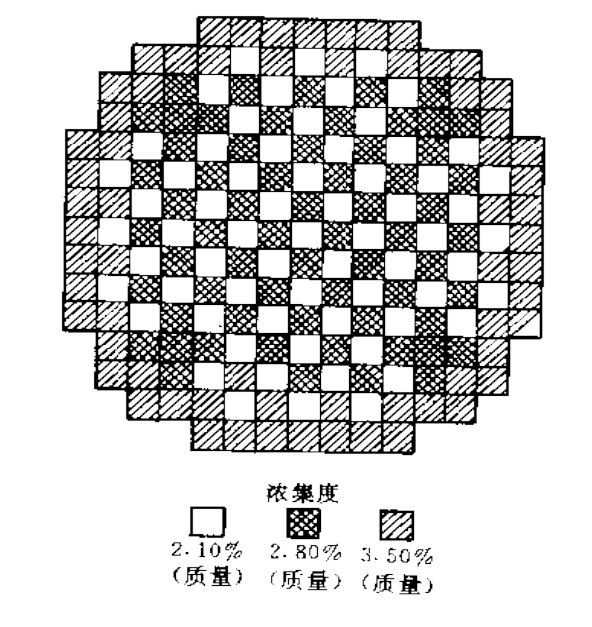
\includegraphics[width=0.7\textwidth]{figures/PWR-fuel-rod.png}
        \caption{压水堆堆芯结构}
        \label{fig:PWR-fuel-rod}
    \end{minipage}
    \hfill
    \begin{minipage}{0.45\textwidth}
        \centering
        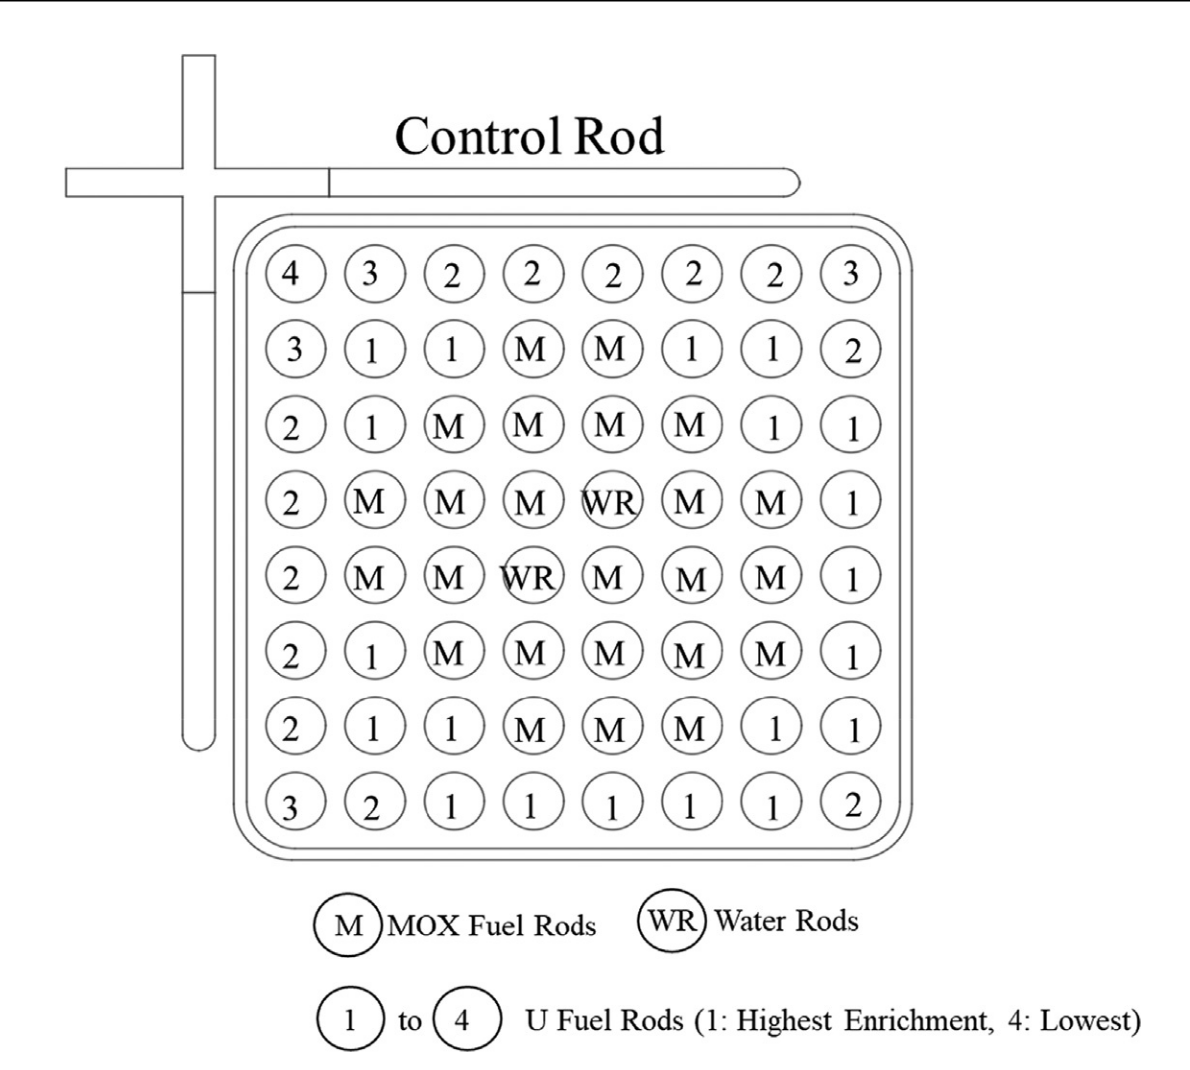
\includegraphics[width=0.8\textwidth]{figures/BWR-fuel-rod.png}
        \caption{沸水堆堆芯结构}
        \label{fig:BWR-fuel-rod}
    \end{minipage}
\end{figure}

同时,如图\ref{fig:PWR-reactor}与\ref{fig:BWR-reactor},压水堆和沸水堆的控制棒位置和驱动装置也有不同之处,压水堆的控制棒驱动装置位于堆芯上方,以获得固有安全性,而沸水堆的控制棒驱动装置位于堆芯下方,以便实现功率调节。

\begin{figure}[htbp]
    \centering
    \begin{minipage}{0.45\textwidth}
        \centering
        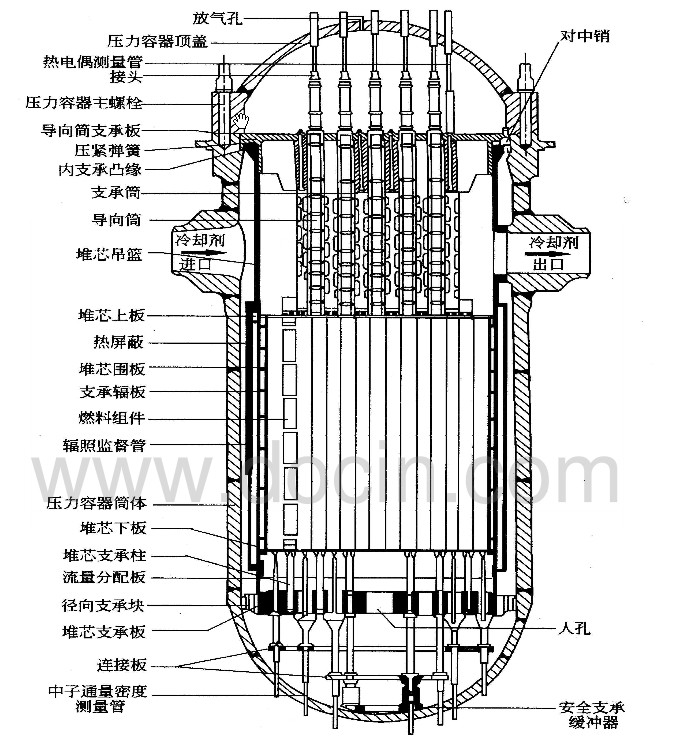
\includegraphics[width=0.8\textwidth]{figures/PWR-reactor.png}
        \caption{压水堆压力容器}
        \label{fig:PWR-reactor}
    \end{minipage}
    \hfill
    \begin{minipage}{0.45\textwidth}
        \centering
        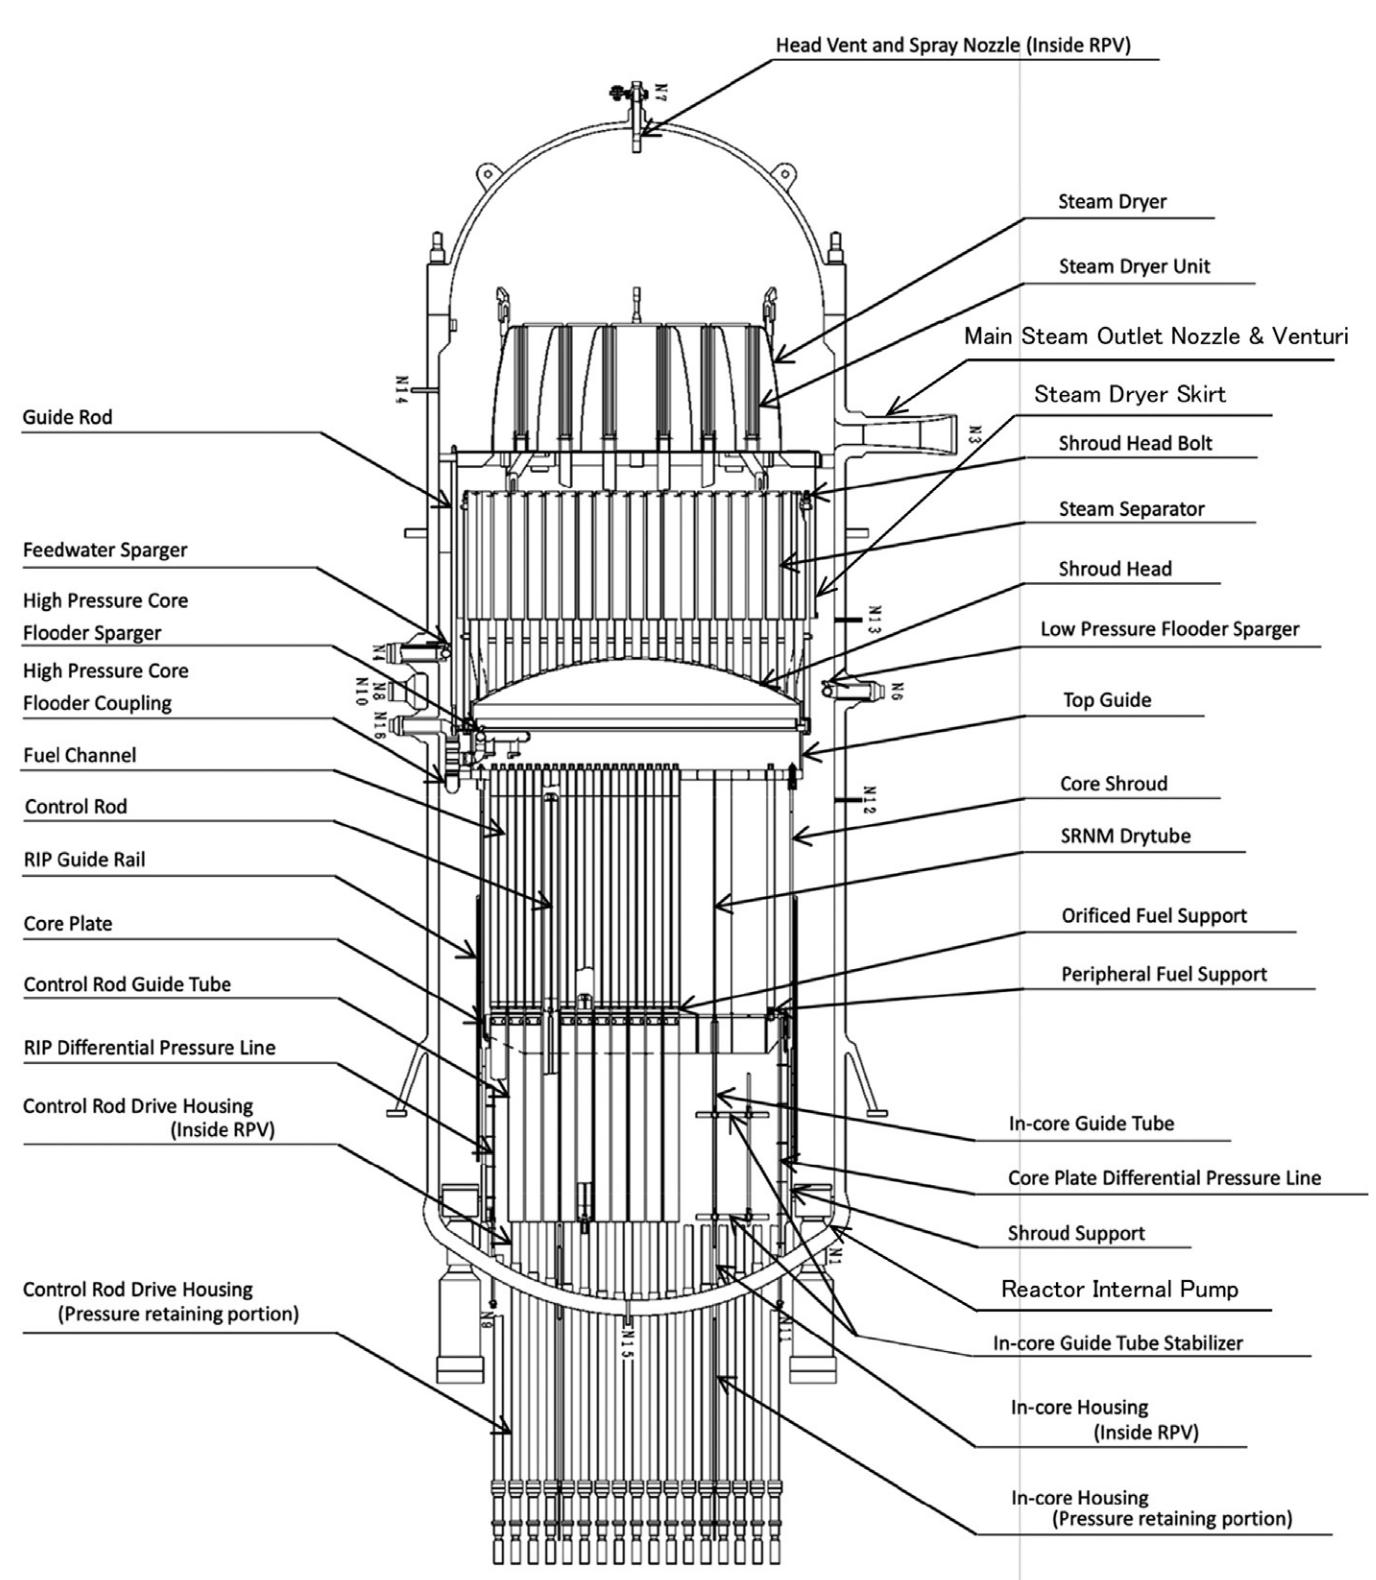
\includegraphics[width=0.7\textwidth]{figures/BWR-reactor.png}
        \caption{沸水堆压力容器}
        \label{fig:BWR-reactor}
    \end{minipage}
\end{figure}

除此之外,如图\ref{fig:BWR-power-distribution},可以知道燃料棒底部的燃料富集度明显小于上部的燃料富集度,采用更低富集度的燃料是为了使得功率更加展平,更容易控制反应性,如图\ref{fig:BWR-power-distribution}所示,采用变化的富集度能够使得燃料棒底部的功率峰降低30\%,且略微提升燃料棒顶部的功率。

\begin{figure}[htbp]
    \centering
    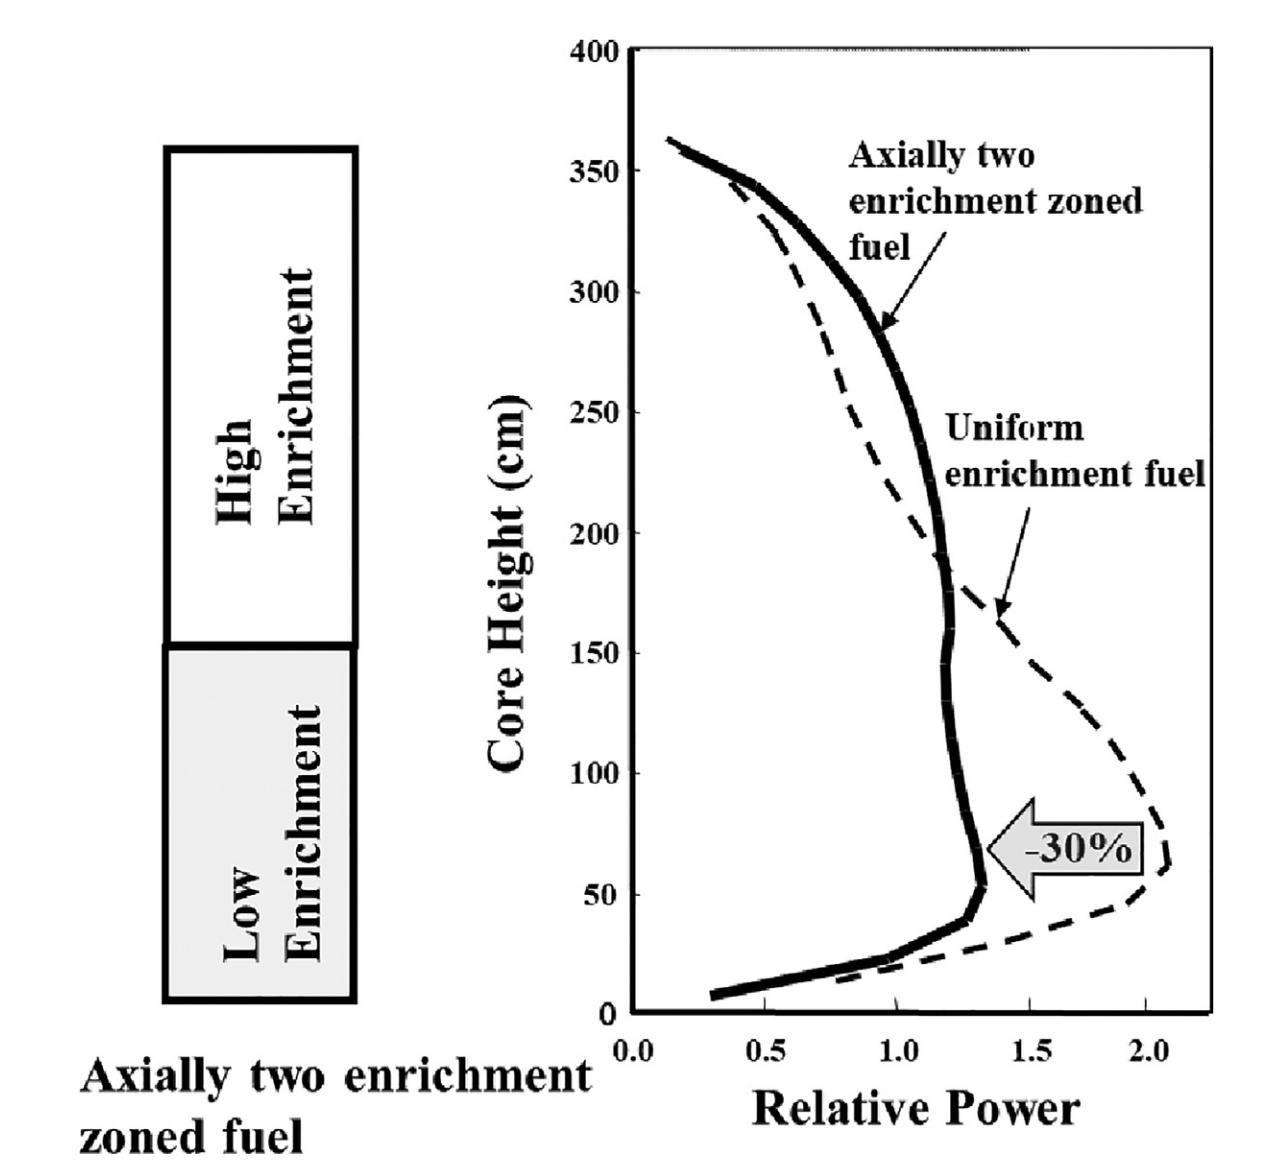
\includegraphics[width=0.6\textwidth]{figures/BWR-power-distribution.png}
    \caption{不同富集度带来的功率变化}
    \label{fig:BWR-power-distribution}
\end{figure}

\section{控制棒形状和反应性控制原理}
\begin{itemize}
    \item \textbf{相同点}:两者都使用控制棒来调节反应堆的反应性,控制核裂变过程。
    \item \textbf{不同点}:
    \begin{itemize}
        \item 在PWR中,如图\ref{fig:PWR-control-rod},控制棒呈星形结构,通过上部的星型骨架操控。这种设计使得PWR的控制棒操作更加简单,但控制效果更加粗糙。
        \item 在BWR中,如图\ref{fig:BWR-control-rod},控制棒为十字形,且只有一根,位于堆芯中心处,将堆芯分为四个小部分。可以在堆芯内部以更灵活的方式插入和抽出,这意味着BWR可以更及时地响应负荷变化。
    \end{itemize}
\end{itemize}

\begin{figure}[htbp]
    \centering
    \begin{minipage}{0.45\textwidth}
        \centering
        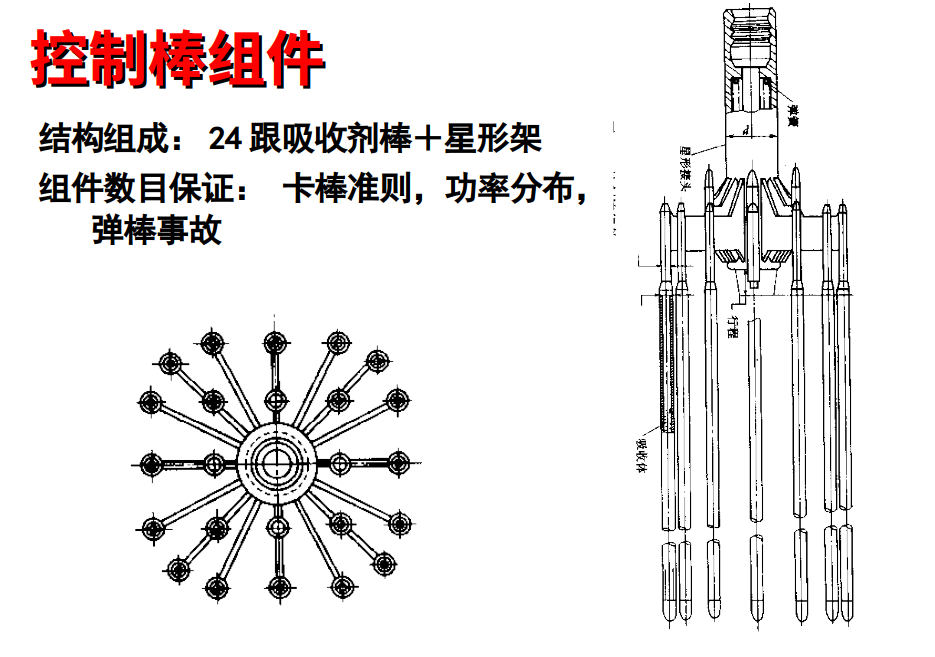
\includegraphics[width=0.7\textwidth]{figures/PWR-control-rod.png}
        \caption{压水堆控制棒}
        \label{fig:PWR-control-rod}
    \end{minipage}
    \hfill
    \begin{minipage}{0.45\textwidth}
        \centering
        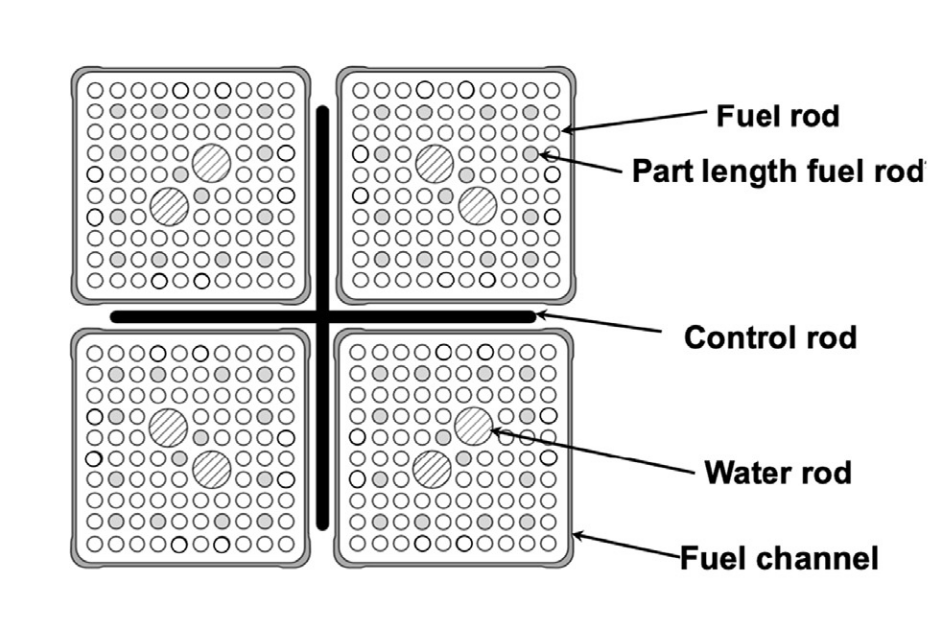
\includegraphics[width=0.7\textwidth]{figures/BWR-control-rod.png}
        \caption{沸水堆控制棒}
        \label{fig:BWR-control-rod}
    \end{minipage}
\end{figure}

沸水堆的控制棒为十字形,且为自下而上插入燃料区。这是因为沸水堆底部的水几乎都为液相,预备反应性更大,从底部插入更容易控制。此外,由于沸水堆上部大部分为蒸汽,核密度较低,且高温蒸汽对控制棒本身及其控制系统更容易产生影响。如果底部的控制棒发生故障导致控制棒掉落,堆芯内的带放射性的冷却水就会发生泄漏,而堆芯得不到冷却,容易发生熔毁等安全事故。

此外,由于压水堆的控制棒为星型架控制的棒状,需要插入燃料组件内部,而沸水堆的控制棒为十字形,只需要插入燃料组件之间的间隙。比较而言,压水堆的控制棒操作更加复杂,但可以达到更加精细的控制效果,可以针对燃料组件内部的中子通量进行控制,而沸水堆的控制棒操作更加简便,但控制效果更加粗糙。

\section{慢化剂作用过程}
\begin{itemize}
    \item \textbf{相同点}:PWR和BWR都使用轻水作为慢化剂,水对中子进行慢化,使其更容易与燃料发生裂变反应。
    \item \textbf{不同点}:
    \begin{itemize}
        \item PWR的水不会在堆芯中沸腾。
        \item BWR的设计允许水在堆芯中部分蒸发,而气态水的核密度更低,慢化能力更弱
    \end{itemize}
\end{itemize}

\section{冷却剂工质的流动传热过程}
\begin{itemize}
    \item \textbf{相同点}:两种反应堆都依赖于流动的水作为冷却剂以带走产生的热量,将核反应释放的热量转变为蒸汽推动汽轮机做功发电。
    \item \textbf{不同点}:
    \begin{itemize}
        \item 如图\ref{fig:PWR-water},PWR利用高压水循环通过蒸汽发生器产生蒸汽,主要通过热交换来完成。水流经堆芯后仍然保持液态,通过蒸汽发生器进行热量交换,使得二回路中的水转换为气态推动汽轮机做功。
        \item 如图\ref{fig:BWR-water},BWR则直接使用堆芯内的水产生蒸汽,减少了热交换的环节,蒸汽直接驱动涡轮发电,但代价是带有放射性的蒸汽直接进入到了汽轮机中,给放射性物质泄漏带来了更多可能性。
    \end{itemize}
\end{itemize}

\begin{figure}[htbp]
    \centering
    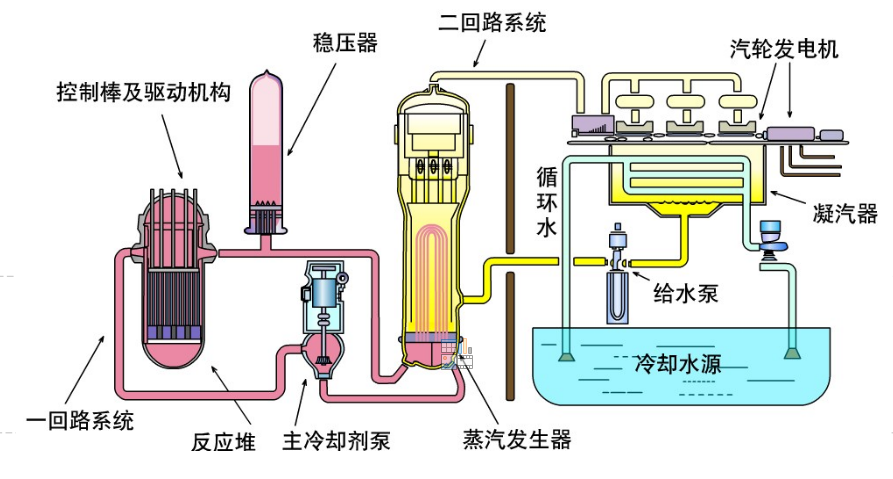
\includegraphics[width=0.9\textwidth]{figures/PWR-water.png}
    \caption{压水堆冷却剂流动示意图}
    \label{fig:PWR-water}
\end{figure}

\begin{figure}[htbp]
    \centering
    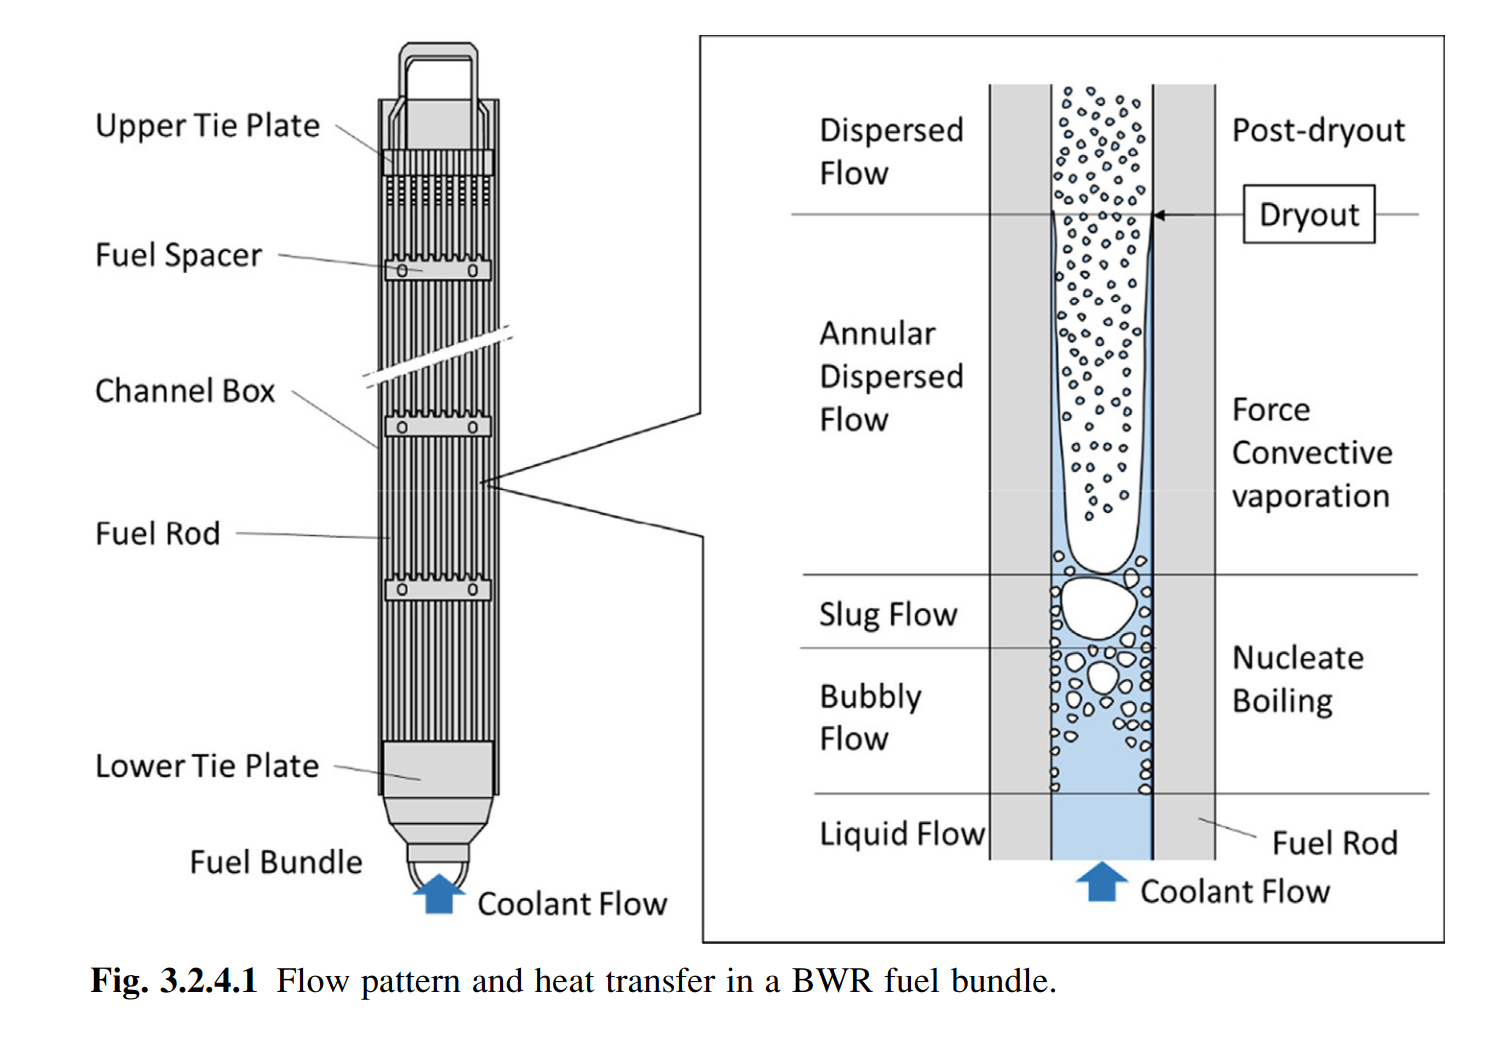
\includegraphics[width=0.7\textwidth]{figures/BWR-water.png}
    \caption{沸水堆冷却剂流动示意图}
    \label{fig:BWR-water}
\end{figure}

\bibliography{cite.bib}

\end{document}